\pdfoutput=1 % only if pdf/png/jpg images are used
\documentclass{JINST}
%\documentclass[options]{article}

\usepackage{url}
\usepackage{lineno}


\begin{document}


\abstract{The ATLAS detector uses a real time selective triggering system to reduce the high interaction rate from 40 MHz to its data storage 
capacity of 1 kHz. A  hardware first level (L1) trigger limits the rate to 100 kHz and a software high level trigger (HLT) 
selects events for offline analysis. The HLT uses the Regions of Interest (RoIs) identified by L1 and 
provided by the Region of Interest Builder (RoIB). The current RoIB is a custom VMEbus based system that operated 
reliably since the first run of the LHC. Since the LHC will reach higher luminosity and ATLAS will increase the complexity and 
number of L1 triggers, it is desirable to have a more flexible and more operationally maintainable RoIB in the 
future. In this regard, the functionality of the multi-card VMEbus based RoIB is being migrated to a PC based RoIB 
 with a PCI-Express card. Testing has produced a system that achieved the targeted rate of 100 kHz.}


\title{The Evolution of the Region of Interest Builder for the ATLAS Experiment at CERN}


%\setpagewiselinenumbers
\linenumbers


\section{Introduction}\label{sec:intro}

The ATLAS \cite{atlas} detector's data acquisition system, illustrated in Figure \ref{fig:atlas_tdaq}, makes use of a multi-tiered trigger to reduce 
bandwidth from the LHC proton bunch crossing rate of 40 MHz
to the \\1 kHz written to disk \cite{evolution}. The first tier (Level-1 or L1) \cite{l1}, implemented in real time with custom electronics, 
makes an early event selection to determine if any objects of interest are present and reduces the data flow to 
100 kHz. The second tier, referred to as the High Level Trigger (HLT) \cite{hlt}, is implemented on a commodity computing cluster running custom triggering software. The HLT uses information from the
hardware based L1 system to guide the retrieval of information from the Readout System (ROS) \cite{ros}. 

Jet, electromagnetic and tau clusters, missing transverse momentum ($E_{\mathrm{T}}^{\mathrm{miss}}$), $\sum E_{\mathrm{T}}$, 
jet $E_{\mathrm{T}}$, and muon candidate information from L1 determine detector Regions of Interest (RoIs) that seed HLT processing. These RoIs are provided to the HLT by a custom VMEbus based system, referred to as the Region of Interest Builder (RoIB) \cite{vme_roib}.
The RoIB collects data from L1 
trigger sources and assembles the data fragments into a complete record of L1 RoIs. These RoIs are made available to the HLT to initiate event processing. In order to improve maintainability and scalability, and to minimize the amount of custom hardware needing to be supported, 
the RoIB will be implemented using commodity server hardware and an interface technology already deployed 
within the ATLAS Trigger and Data Acquisition (TDAQ) system. The approach of implementing the RoIB functionality in software has been investigated in the past 
and the conclusion at that time was that a software based approach is possible but requires a higher rate readout card \cite{swroib_past}. 
Since data readout cards operating at high rates became available and the capabilities of computers have improved with the increase 
in CPU clock speed and number of cores, it became possible to implement the RoIB functionality using a PC based approach. 
The PC based RoIB must duplicate the functionality of the VMEbus based RoIB which means that the PC based solution must receive and assemble the
individual L1 fragments, and pass them as a single L1 result to the HLT. Modern computers have multicore CPU architectures 
with the possibility of running multi-threaded application, a feature which is being fully exploited in the RoIB software to achieve 
the desired performance of 100 kHz over 12 input links for fragment sizes of 400 bytes.  
This paper describes the evolution of the RoIB from the VMEbus based system to the PC based system and gives details on the hardware, 
firmware, and software designs used to achieve the full RoIB functionality. 



\begin{figure}[tbp] % figures (and tables) should go top or bottom of
                    % the page where they are first cited or in
                    % subsequent pages
\centering
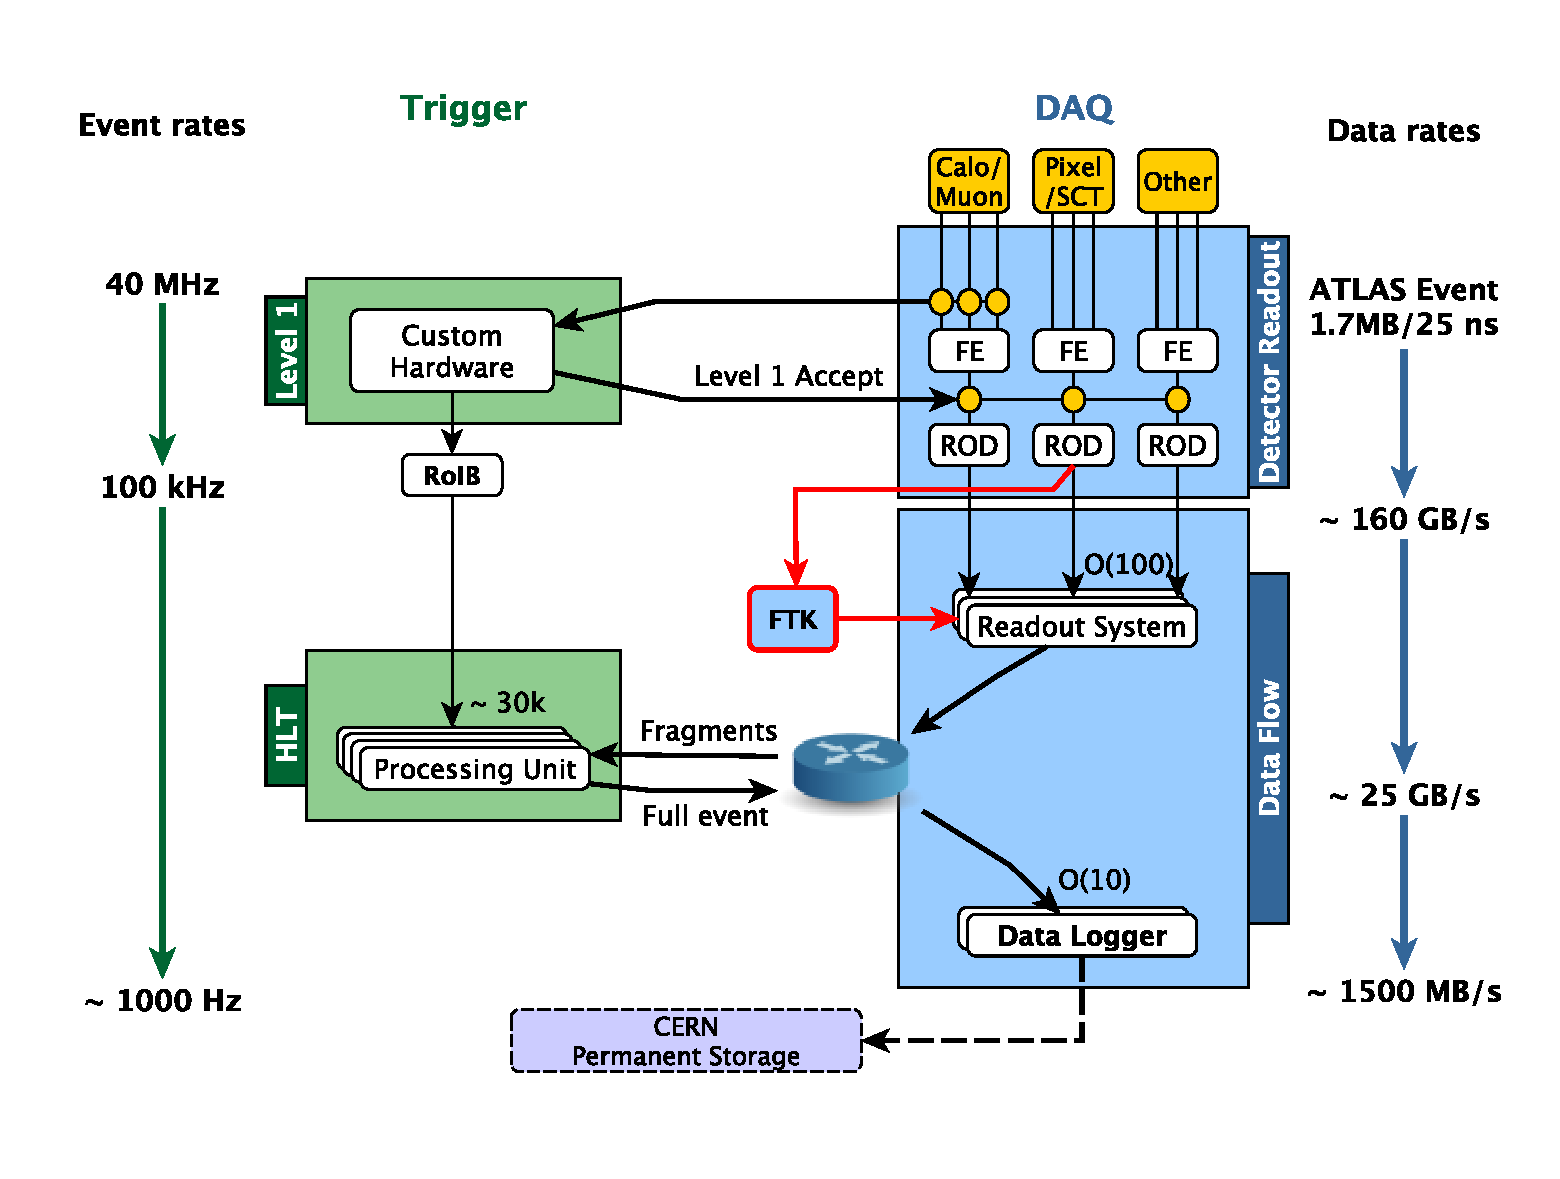
\includegraphics[width=.9\textwidth]{figures/tdaqFullNew2015}
\caption{ATLAS TDAQ Architecture.}
\label{fig:atlas_tdaq}
\end{figure}



%\section{ATLAS TDAQ System }\label{sec:tdaq}

%\subsection{Challenges}\label{sec:tdaq_chal}

%\subsection{Architecture}\label{sec:tdaq_archi}


\section{VMEbus based RoIB}\label{sec:roib}

\subsection{Hardware implementation}\label{sec:roib_current}

The RoIB is implemented as a custom 9U VMEbus system that includes a controller which configures and monitors the system along with custom cards 
that receive and assemble the event fragments and send them to the HLT. Figure \ref{roib_run1} shows a block of the RoIB and 
its connection to external systems.
%\footnote{Note the L2 Supervisor farm from Run-1 has evolved to a commodity server PC running the HLTSV application.}.

\begin{figure}[tbp] % figures (and tables) should go top or bottom of
                    % the page where they are first cited or in
                    % subsequent pages
\centering
\includegraphics[width=.65\textwidth]{figures/RoIB_context_v2.png}
\caption{Block scheme of the RoI Builder and overview of connections to external systems.  The
custom input and builder cards and the controller, a commercially available single board computer,
are installed in a single 9U VMEbus crate. The controller connects to the Control Network to interact with the rest of the 
data acquisition system.}
\label{roib_run1}
\end{figure}

The RoIB contains four input cards and uses one builder card in the Run-2 configuration. Each input card accepts three inputs from 
L1 subsystems. 
The builder card assembles the input data of the events and passes the results via two optical links 
to another receiver card in a PC running the HLT supervisor (HLTSV) application. The receiver card in the HLTSV is a TILAR card \cite{tilar}
 that implements four PCIe Gen1 lanes to interface with the two optical links. The HLTSV manages the HLT processing farm by using L1 results provided by the RoIB, retrieves events from the ROS, assigns events to HLT farm nodes, and handles event bookkeeping including requesting removal of data from ROS storage when no longer required. 

The fragments received by the RoIB are identified by a 32 bit identifier, the extended L1 ID (L1ID). 
The RoIB input cards use the L1ID and the number of outputs enabled to assign keys to the various fragments and send them to the output channel in the builder card that was 
assigned that key value. The input data is transferred over a custom J3 backplane. The backplane operates at 20 MHz and transfers 16 data bits per 
clock cycle simultaneously for up to 12 inputs. The total maximum data throughput is therefore 480 MB/s, 40 MB/s per input.  
The maximum size of any single fragment is limited to 512 bytes imposed by resources available in the FPGA firmware. The current RoIB input 
links are listed in Table \ref{tab:roib_links}.

\begin{table}[tbp]
\caption{L1 input sources to the RoIB.}
\label{tab:roib_links}
\smallskip
\centering
\begin{tabular}{|c|c|}
\hline
Source & Links\\
\hline
Central Trigger Processor (CTP)  & 1  \\
L1 calorimeters (e/$\gamma$, $\tau$, jet, $\sum E_\mathrm{T}$) & 6  \\
Muon Trigger to CTP Interface (MUCTPI) & 1  \\
Topological processor (L1Topo) & 2  \\
Spare & 2 \\
\hline
\end{tabular}
\end{table}

\subsection{System Performance and Evolution}\label{sec:roib_limit}

The custom VMEbus based RoIB operated reliably during the first run of the LHC, however, it is desirable to have a more flexible RoIB. 
In addition, the RoIB is getting close to its design limitation, as seen 
in Figure \ref{fig:cern_robinnproib}. For fragments of 400 bytes and inputs from eight L1 systems, referred to as channels, the current RoIB rate limit is 60 kHz which is below the required 100 kHz at 
L1. While the current fragment size coming from L1 are around 160 bytes, the sizes are expected to grow due to the increase of instantaneous 
luminosity and the complexity of L1 triggers. The current VMEbus system will be replaced by a PCI-express card hosted in the HLTSV PC with the 
possibility to upgrade the commodity hardware (e.g. ability to upgrade CPUs). 
The new configuration simplifies the readout architecture of ATLAS. The targeted rate for event building is 100 kHz over 12 input channels for 
fragment sizes in the order of 400 bytes.

\section{PC based RoIB}\label{sec:roib_new}

 A custom PCIe card developed by the ALICE collaboration, the Common ReadOut Receiver Card (C-RORC) \cite{alice}, was deployed as an 
upgraded detector readout interface within the ATLAS ROS with ATLAS specific firmware and software called the RobinNP \cite{crorc}. 
The new PC based RoIB uses the RobinNP firmware and a dedicated API to facilitate the implementation of the RoIB functionality 
on a commodity PC. In this section, we describe the C-RORC hardware as well as the RobinNP firmware, API, and the event building software. 
\subsection{The Common Readout Receiver Card}\label{sec:crorc}

The C-RORC implements 8 PCIe Gen1 lanes with 1.4 GB/s bandwidth to the CPU fed via 12 optical links each running 200 MB/s on 3 QSFP transceivers. It utilizes a single Xilinx Virtex-6 series FPGA that handles data input from the 12 links and buffers the data in two on-board DDR3 memories. It is also capable of processing and initiating DMA transfer of event data from the on-board memory to its host PC's memory. The major components of the C-RORC are annotated 
in the picture shown in Figure \ref{fig:crorc}.


\begin{figure}[tbp] % figures (and tables) should go top or bottom of
                    % the page where they are first cited or in
                    % subsequent pages
\centering
\includegraphics[width=\textwidth]{figures/crorc.png}
\caption{Photo of the C-RORC board with the major components and features annotated \cite{crorc}.}
\label{fig:crorc}
\end{figure}

\begin{figure}[tbp] % figures (and tables) should go top or bottom of
                    % the page where they are first cited or in
                    % subsequent pages
\centering
\includegraphics[trim = 0cm 0cm 0cm 2.5cm, clip, width=.71\textwidth]{figures/RobinNP_Firmware}
%\includegraphics[width=.6\textwidth]{figures/Firmware.jpg}
%\includegraphics[width=.8\textwidth]{figures/AReducedBlockDiagram.png}

\caption{RobinNP firmware organization
and  flow  of  data  from  host  CPU  to  the
firmware  (by  means  of  programmed  I/O)
and from the firmware to the host memory
(by means of DMA).}
\label{fig:robinnp_fw}
\end{figure}

\subsection{Readout System Firmware \& Software}\label{sec:crorc_fw}

The RobinNP firmware used for the RoIB is identical to that used in the ATLAS ROS\cite{ros}. As shown in 
the schematic of Figure \ref{fig:robinnp_fw}, the logic is divided into two functional blocks, known as sub-ROBs, 
each servicing six input links and one DDR3 memory module. Event data fragments arriving via a link are subjected 
to a range of error checks before being stored in the memory module for the relevant sub-ROB. At the same time a token
representing the address of a region of the memory, referred to as a page, is passed to a listening software process via 
a `FIFO duplicator'. To avoid a costly read across the PCIe bus, data is continuously streamed from firmware to 
software via a chain of firmware and software FIFOs. Notification of new data arriving in the software FIFO is managed via coalesced 
interrupts to allow for efficient use of CPU resources.
For the RoIB application, the receipt of page information immediately triggers a DMA of fragment data from the RobinNP memory into 
the host PC memory. The fragments are then passed via a queue (one per sub-ROB) to the RoIB process along with any relevant fragment 
error information. A schematic of this shortened dataflow path is presented in Figure \ref{fig:roib_swfw}. 
The API for the RoIB process consists of these queues, return queues for processed pages now available for re-use and 
a configuration interface. The software is implemented with multiple threads each handling specific tasks such as supply of free pages, receipt
of used pages, DMA control and bulk receipt of fragment data.


\begin{figure}[tbp] % figures (and tables) should go top or bottom of
                    % the page where they are first cited or in
                    % subsequent pages
\centering
%\includegraphics[width=.6\textwidth]{figures/roib_firmware.png}
\includegraphics[trim = 0cm 0cm 0cm 5cm, width=.7\textwidth]{figures/RobinNP_Software}
\caption{Layout of the readout system firmware and software specific to the RoIB.}
\label{fig:roib_swfw}
\end{figure}

\subsection{RoIB Software}\label{sec:crorc_sw}

The HLTSV is a multi-threaded application that obtains a L1 result from a variety of possible input sources and exchanges information with the 
rest of the HLT computing farm. 
%Data Collection Managers (DCM). The DCM is the application running on each HLT computing node that tells the HLTSV if the event has been rejected, successfully built, or timed out and also requests the data from the ROS. In this case, 
For the RoIB, the L1 source is a RobinNP interface that performs fragment assembly and is used as a plug-in to the HLTSV application.
The RobinNP plug-in has two receive threads, each 
thread services six channels by pulling fragments from the RobinNP on-board memories to the host PC.
Fragments with the same L1ID are copied 
to a contiguous memory space and a queue of completed events is prepared. 
Upon request by the HLTSV, a pointer to the contiguous memory space is passed back to the 
HLTSV process for further handling. In order to optimize concurrent access to RoIB data structures, containers from the  Intel 
threading building block (TBB) library were used. These containers allow multiple threads to concurrently access and update items 
in the container while maintaining high performance.  


\section{Prototype Tests}\label{sec:perf}

In order to understand the requirements for the underlying server PC, a validation system based on Intel(R) Xeon(R) CPU E5-1650 v2 
@ 3.5 GHz with six cores is being used to perform tests of the PC based RoIB. 
The goal is to perform software based fragment assembly at a rate of 100 kHz over 12 channels for a typical 
fragment size of 400 bytes. The current system offers flexibility in terms of the fragment size allowed which was not the case in the 
VMEbus based RoIB. The initial tests were performed with a standalone application that implements a minimal interface for event building. 
Once the system was validated, the relevant code modules were integrated into an HLTSV process running within the full ATLAS TDAQ 
software suite with appropriately scaled test hardware to represent the remaining elements of the system.

\subsection{Standalone Tests}\label{sec:perf_alone}

The goal was to test input/output bandwidth limitations of the RobinNP and the rate of event building. Initial performance testing used 
a standalone RobinNP application and an external source that emulates the L1 trigger data 
in the form of 32-bit word fragments with 12 channels. In this test, the host PC was running the assembly routine with a single threaded application.  Figure \ref{fig:cern_robinnproib} shows the input rate without 
event building as a function of fragment size. For 400 byte fragments the input rate to the RobinNP is 215 kHz. 
The same figure 
shows the event building rate which is 150 kHz. This performance shows that the event building 
at the required rate of 100 kHz with 12 channels is achievable in a standalone application.  


\begin{figure}[tbp] % figures (and tables) should go top or bottom of
                    % the page where they are first cited or in
                    % subsequent pages
\centering
\includegraphics[width=.7\textwidth]{figures/cern_robinnproib.pdf}
\caption{Rate as a function of the fragment size (in bytes) with external source that emulates the L1 trigger input. 
The rates shown are for the input rate to the RobinNP without event building (EB) (triangle), rate with EB (circle), and 
for comparison, the current VMEbus RoIB rate is also shown (square).  }
\label{fig:cern_robinnproib}
\end{figure}


\subsection{Full System Tests}\label{sec:perf_tdaq}

Since the HLTSV is performing tasks other than the event building, there is overhead associated with additional operations 
that reduces the performance. For this reason, we use the full ATLAS TDAQ software in a test environment that emulates the major components of the ATLAS data acquisition system shown in Figure \ref{fig:atlas_tdaq}. The setup includes an emulated input from L1 trigger sources, 
the HLTSV and other PCs to simulate the HLT computing farm, and the ROS that buffers the full event data. 
 In this test setup, an external source sends data that emulates L1 RoIs via 12 links connected to the 
RobinNP hosted by the HLTSV. When the HLTSV requests a built RoI event, the software RoIB plug-in provides the RoI event which will be used 
to seed requests for the event data to be processed.
 Figure \ref{fig:partition} shows an event building rate of 110 kHz measured with 400 byte fragments with the HLTSV application in a setup close to the ATLAS TDAQ system. 

\begin{figure}[tbp] % figures (and tables) should go top or bottom of
                    % the page where they are first cited or in
                    % subsequent pages
\centering
\includegraphics[width=.98\textwidth]{figures/12ch.png}
\caption{Screenshot of a monitoring tool which shows the HLTSV processing rate using the ATLAS TDAQ software .}
\label{fig:partition}
\end{figure}


\section{Outlook}\label{sec:outlook}

The RoIB will evolve from the VMEbus based system to the PC based system using a PCI-Express card and firmware shared with the 
ATLAS ROS. The new system will add flexibility and improve maintainability of the ATLAS TDAQ system. As the technology 
evolves, the PCs and CPUs can be upgraded and more channels can be included by adding more RobinNP cards while maintaining high 
readout rates. A full integration test of the readout performance of the ATLAS TDAQ system with the PC based RoIB will be performed 
during the 2015-2016 LHC winter shutdown in preparation for a system evolution.


%\textbf{Use of this architecture for the ROS push-push mode?}
%\textbf{Run 3 and beyond -> necessary}



%\acknowledgments

%We would like to thank the ROS team for facilitating the tests of the PC based RoIB at CERN as well as reviewing the RoIB software and 
%help in improving it. We particularly thank William Panduro Vazquez and Wainer Vandelli from the team. 



\begin{thebibliography}{9}

\bibitem{atlas}
ATLAS Collaboration, \emph{The ATLAS experiment at the CERN Large Hadron Collider}, \jinst{3}{2008}{S08003}.

\bibitem{evolution}
 N. Garelli (on behalf of the ATLAS Collaboration),
\emph{The Evolution of the Trigger and Data
Acquisition System in the ATLAS Experiment},
{J. Phys.: Conf. Ser.
513 (2014) 012007.}



\bibitem{l1}
ATLAS Collaboration, \emph{ATLAS Level-1 Trigger: Technical Design Report}, 
{ATLAS-TDR-12}, 1998


\bibitem{hlt}
ATLAS Collaboration,
\emph{ATLAS, High-Level Trigger, Data Acquisition and Controls} \href{https://cds.cern.ch/record/616089}{https://cds.cern.ch/record/616089}
\emph{CERN/LHCC/2003-022}, CERN Geneva 2003.






\bibitem{ros}
A. Borga et al.,\emph{Evolution of the ReadOut System of the ATLAS experiment}, in proceedings of
\emph{Technology and Instrumentation in Particle Physics 2014}, June, 2--6, 2014 Amsterdam, the Netherlands
\pos{PoS(TIPP2014)205}.



\bibitem{vme_roib}
R. Blair et al.,
\emph{The ATLAS High Level Trigger Region of Interest Builder},
\jinst{3}{2008}{P04001} 


\bibitem{swroib_past}
R. E. Blair et al., \emph{ATLAS TDAQ dataflow: Software RoI builder status report}, {ATL-DQ-TR-0020}, 2012


\bibitem{l1ttc}
S. Ask et al., \emph{The ATLAS central level-1 trigger logic and TTC system}, \jinst{3}{2008}{P08002}.


%\bibitem{slink}
%O. Boyle, R. McLaren, E. Van der Bij, \emph{
%The S-LINK Interface Specification}, \url{http://hsi.web.cern.ch/HSI/s-link/}


\bibitem{tilar}
CERN, \url{http://www.cerntech.hu/products/15-tilar-express.html}, October 15, 2015


\bibitem{alice}
H. Engel,U. Kebschull (For the ALICE Collaboration),
\emph{Common read-out receiver card for ALICE Run2},
\jinst{8}{2013}{C12016}.

\bibitem{crorc}
A. Borga et al., \emph{The C-RORC PCIe Card and its Application in the ALICE and ATLAS Experiments}, \jinst{10}{2015}{C02022}.


%\bibitem{L1}
%ATLAS Collaboration, \emph{ATLAS level-1 trigger: Technical Design Report},





\end{thebibliography}
\end{document}
